%%%%%%%%%%%%%%%%%%%%%%%%%%%%%%%%%%%%%%%%%%%%%%%%%%%%%%%%%%%%%%%%%%%%%%%%%%%%%%%
%
% Tommy P. Keane
% Master of Science Thesis
% Department of Electrical and Microelectronic Engineering
% Rochester Institute of Technology
%
% April 2011
%
%
%
% Funded By: Lenel Systems Inc., A UTC Fire & Security Corporation
%
% Algorithm Intellectual Property Owned By: Lenel Systems Inc.
%
%
% http://www.tommypkeane.com
%
%%%%%%%%%%%%%%%%%%%%%%%%%%%%%%%%%%%%%%%%%%%%%%%%%%%%%%%%%%%%%%%%%%%%%%%%%%%%%%%

%%%%%%%%%%%%%%%%%%%%%%%%%%%%%%%%%%%%%%%%%%%%%%%%%%%%%%%%%%%%%%%%%%%%%%%%%%%%%%%
%
% CHAPTER 1
%
% PREAMBLE: Introduction
%
%%%%%%%%%%%%%%%%%%%%%%%%%%%%%%%%%%%%%%%%%%%%%%%%%%%%%%%%%%%%%%%%%%%%%%%%%%%%%%%


%%%%%%%%%%%%%%%%%%%%%%%%%%%%%%%%%%%%%%%%%%%%%%%%%%%%%%%%%%%%%%%%%%%%%%%%%%%%%%%
% BEGIN DOCUMENT
Before delving into the depths the algorithm, its development, its implications, its contributions, its results, and its potential future, there needs to be an introduction to what has been, and what is trying to be, achieved here. Mathematics and programming are languages, they are functional, and they are tools to serve a purpose. Without understanding that purpose, without preparation and a solid foundation, there would be nothing but a set of facts and figures susceptible to misinterpretation. The core of the WFMI algorithm is in its implementation through a thorough understanding of the underlying mathematics and practical considerations. A lot of the following discussion is then focused on explaining where the application of these operations follows from, and why and when it succeeds or fails. In order to maintain a clear and consistent understanding the following terms and phrasings will be used.

A \textbf{scene} is understood here as the real-world location being imaged, and the camera imaging the scene is known as the \textbf{view} (of the scene). The output of the camera is understood to be a digital tri-chromatic video composed of tri-chromatic (typically RGB) \textbf{frames}. The most important term will be the \textbf{overlap} between views. In this context we are defining \textbf{overlap} to mean the regions within the views' frames which have imaged the \textit{same existing region} within the scene. Characteristics of imaging geometry will not always allow for identical overlap regions in the frames, but our definition will apply to the understanding that there is real-world correspondence between the objects from the scene imaged onto the frames through the multiple views.

In order to maintain consistent terminology across the development and implementation, MATLAB\textsuperscript{\textregistered} notation for image sizing will be followed, where each image is of size $\mathfrak{m}\times\mathfrak{n}\times\mathfrak{p}$. The row, column, and channel indices will come from the following closed sets, respectively: $[1,\mathfrak{m}]$, $[1,\mathfrak{n}]$, and $[1,\mathfrak{p}]$. While it is more mathematically apt to model each frame (image) from each view as the realization of a random process (the camera capturing the scene), we simplify the terminology and understanding to assume each frame is a discrete random variable that is a 3-Dimensional (3-D) set of $b$-bit intensity values. To characterize these random variables (R.V.) we develop a model of their 1-D Probability Mass Function (PMF) based on features (a 2-D array) from the images. Each image's PMF is then an approximation of the characterization of the real-world scene; which under a continuous R.V. model would be its Probability Density Function (PDF). It is understood, and applied in development, that each image has come from a projection, sampling, and quantization of the scene at that view, as shown in part in Figure \ref{CameraModel}.

\begin{figure}[!h]
\centering
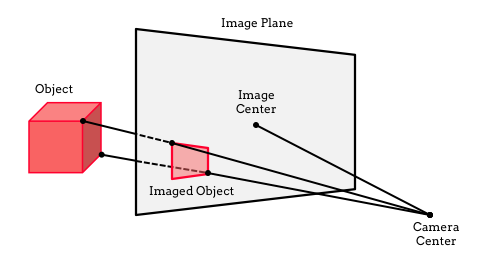
\includegraphics[width=.7\columnwidth]{CameraModel}
\caption{Projective Camera System Model}
\label{CameraModel}
\end{figure}

%%%%%%%%%%%%%%%%%%%%%%%%%%%%%%%%%%%%%%%%%%%%%%%%%%%%%%%%%%%%%%%%%%%%%%%%%%%%%%%
% END OF DOCUMENT
